% CVPR 2023 Paper Template
% based on the CVPR template provided by Ming-Ming Cheng (https://github.com/MCG-NKU/CVPR_Template)
% modified and extended by Stefan Roth (stefan.roth@NOSPAMtu-darmstadt.de)

\documentclass[10pt,twocolumn,letterpaper]{article}

%%%%%%%%% PAPER TYPE  - PLEASE UPDATE FOR FINAL VERSION
\usepackage{cvpr}      % To produce the REVIEW version


% Include other packages here, before hyperref.
\usepackage{graphicx}
\usepackage{amsmath}
\usepackage{amssymb}
\usepackage{booktabs}
\usepackage{textcmds}



% It is strongly recommended to use hyperref, especially for the review version.
% hyperref with option pagebackref eases the reviewers' job.
% Please disable hyperref *only* if you encounter grave issues, e.g. with the
% file validation for the camera-ready version.
%
% If you comment hyperref and then uncomment it, you should delete
% ReviewTempalte.aux before re-running LaTeX.
% (Or just hit 'q' on the first LaTeX run, let it finish, and you
%  should be clear).
\usepackage[pagebackref,breaklinks,colorlinks]{hyperref}


% Support for easy cross-referencing
\usepackage[capitalize]{cleveref}
\crefname{section}{Sec.}{Secs.}
\Crefname{section}{Section}{Sections}
\Crefname{table}{Table}{Tables}
\crefname{table}{Tab.}{Tabs.}


%%%%%%%%% PAPER ID  - PLEASE UPDATE
\def\cvprPaperID{*****} % *** Enter the CVPR Paper ID here
\def\confName{CVPR}
\def\confYear{2023}


\begin{document}

%%%%%%%%% TITLE - PLEASE UPDATE
\title{Team 81: Detecting AI generated images}

\author{
Anthony John Dsouza\\
7053485\\
\and
Eva Morgan Toulouse Gavaller\\
7056847\\
%\and
%Name 3\\
%Matriculation 3\\
}
\maketitle

%%%%%%%%% BODY TEXT
\section{Task and Motivation}
% test \cite{zhangCommonSenseReasoning2025}
\subsection{Task statement \& Motivation}
With recent advancements in AI, generative models like the transformer, diffusion, SSMs make use of vast \& diverse training data to generate text, images and audio indistinguishable from human generated data. These technologies have found use in machine translation, human machine interaction, image inpainting, text to video / image generation, etc. While many of these applications are beneficial to society, some bad actors use these tools for nefarious purposes, like spreading misinformation and revenge pornography. 
During this project we inted to explore methods to detect deepfakes and AI-generated media. To accomplish this, we intend to collect an AI-generated visual dataset, and annotate it. 

We have 2 closely related ideas that we can look to implement

\begin{enumerate}
	\item Idea 1 : Vision Language Model to detect AI generated images using reasoning
	\item Idea 2 : Interpreting finetuned ViT hidden states
\end{enumerate}

%We will then train ViT-based model to detect deepfakes as well as train a VL model [PaliGemma, phi, etc] to reason with features extracted by an image encoder to determine why a provided image or video is predicted as real or fake. We are very curious about which features classifiers and detectors focus on in deepfake prediction. 
%Therefore, we plan to use methods for interpretabllity such as attention rollout and Sparse Auto-Encoders (SAEs) to better understand our model. 

%- would like to explore methods to detect deepfakes / ai generated media 
%- collect ai generated visual dataset, annotate it for 


%-- train VIT based model to detect deepfakes

%-- train a VL model [PaliGemma, phi, etc] to reason with features extracted by image encoder and why provided image / video is real or fake

%-- what features do classifieVision Language Model to detect AI generated imagesrs / detectors focus on? [look at attention rollout, SAE features, any more techniques?]



\subsection{Related work}
Most common approaches use a simple setup, by fine-tuning a CNN / Vision Transformer \cite{dosovitskiyImageWorth16x162021} with some simple augmentations on datasets like \cite{dolhanskyDeepFakeDetectionChallenge2020, rosslerFaceForensicsLargescaleVideo2018, zhengBreakingSemanticArtifacts2024, liCelebDFLargeScaleChallenging2020}. The approach considered here is `classification', where the detector tries to identify artifacts generated by the generators. The DeepFake Detection challenge by Meta and Kagggle \footnote{\href{https://ai.meta.com/datasets/dfdc/}{DeepFake Detection Challenge}} saw many submissions using the above approaches with the best performing submission \cite{seferbekovDeepfakeDetectionChallenge} being an ensemble of many models with augmentations and more importantly face warping artifacts \cite{liExposingDeepFakeVideos2019}. Other approaches used \cite{yunCutMixRegularizationStrategy2019a, hendrycks*AugMixSimpleData2019, zhangMixupEmpiricalRisk2018a} for improved generalization.

In \cite{feiExposingAIgeneratedVideos2021}, the authors use motion magnification to amplify imperceptible movements in videos, making them observable. Initially developed to detect subtle vibrations in structures like high-rise buildings and bridges, this technique revealed that synthetic videos exhibit a higher flicker rate compared to real videos. To analyze these differences, the authors use InceptionV3 \cite{szegedyRethinkingInceptionArchitecture2015} as the backbone for extracting spatial features from video frames and an LSTM \cite{hochreiterLongShortTermMemory1997} to process temporal data, enabling effective discrimination between real and synthetic videos based on motion patterns.

In \cite{zhangCommonSenseReasoning2025}, authors reframe deepfake detection as a common sense reasoning task, aiming to address limitations of image classifiers that fail to identify subtle inconsistencies, such as unnatural skin tones or duplicate features like double eyebrows. Using a language model, the method reasons whether an image is real or fake, specifically highlighting inconsistencies in the temporal domain. This allows for a more nuanced analysis of visual content beyond standard detection techniques. For this, the authors use a BLIP \cite{liBLIPBootstrappingLanguageImage2022} backbone, integrating a BERT \cite{devlinBERTPretrainingDeep2019} like text encoder and a Vision Transformer \cite{dosovitskiyImageWorth16x162021} based image encoder, with cross-modal attention mechanism for vision language grounding between the two modalities. The textual outputs generated by the encoders are then fed into the language model that reasons if the provided image is real or fake.

SurFake's \cite{ciamarraDeepfakeDetectionExploiting2024} approach is based around concept that pixels in an image contain critical information about scene geometry and the acquisition process, which is often altered by deepfake generators, leaving detectable traces. By analyzing these pixel-level changes, SurFake aims to identify manipulations that traditional methods might overlook. The detection pipeline consists of three key steps- First, it performs face detection and extraction to isolate the relevant facial region. Next, a Global Surface Descriptor, based on UpRightNet \cite{xianUprightNetGeometryAwareCamera2019}, is used to capture the geometrical characteristics of the extracted face. Finally, these features are processed by a convolutional neural network (CNN), which analyzes the geometric data to determine whether the image has been manipulated, enabling robust deepfake detection.

\cite{huangSIDASocialMedia2025} created the Social Media Image Detection Dataset, comprising 300,000 images that include real, AI-generated, and tampered images. This dataset emphasizes broad diversity and realism to ensure it reflects the complexities of images encountered on social media platforms, providing a robust resource for developing and evaluating detection models. For detection, the authors improve on the LISA \cite{laiLISAReasoningSegmentation2024} model by introducing two new tokens to its vocabulary: one for detection \texttt{<DET>} and one for segmentation \texttt{<SEG>}. The model takes an image and a prompt, such as “Can you identify if this image is real, fully synthetic, or tampered?” as input. It then generates a text description explaining its reasoning, while the last hidden layer contains the two additional tokens. The \texttt{<DET>} token identifies whether the image is manipulated, and if tampering is detected, the \texttt{<SEG>} token highlights the specific regions that have been altered, enabling precise localization of modifications.

\subsection{Challenges}
\begin{figure}[h]
	\centering
	\begin{subfigure}{0.45\columnwidth}
		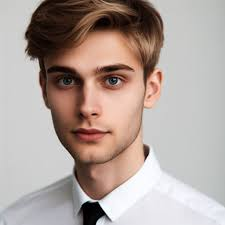
\includegraphics[width=\textwidth]{/home/tororo.in/Desktop/UnFakeIt/paper/face.jpeg}
		\caption{Image has unnatural lighting}
	\end{subfigure}
	\hfill
	\begin{subfigure}{0.45\columnwidth}
		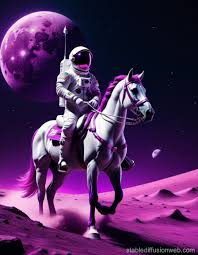
\includegraphics[width=\textwidth]{/home/tororo.in/Desktop/UnFakeIt/paper/horse.jpeg}
		\caption{Image defies logic as astronauts do not ride horses in space / on other planets}
	\end{subfigure}
	
\end{figure}


A significant portion of methods for deepfake detection systems were built before diffusion \cite{hoDenoisingDiffusionProbabilistic2020} was introduced- mainly due to the fact that training these models was computationally expensive. Soon, \cite{dhariwalDiffusionModelsBeat2021} showed that diffusion-based image generation models were better at image generation while being stable in comparison to their counterparts.\cite{rombachHighResolutionImageSynthesis2022}, \cite{lipmanFlowMatchingGenerative2023} build on this for improved generation, with methods developed to control the generation process like \cite{ruizDreamBoothFineTuning2023, zhangAddingConditionalControl2023} and using fewer steps for denoising as in \cite{lipmanFlowMatchingGenerative2023}. All these result in hyperrealistic image generation with few artifacts, making the process of detecting deepfakes highly difficult. 


\section{Goals}

\subsection{Challenges we aim to address}
%\subsubsection{Idea 1 : Vision Language Model to detect AI generated images}
%Our goal for this project is two-fold. First, we aim to address the lack of data and research on AI-generated and tampered images created using newer methods such as diffusion models. Second, we aim to use mechanistic interpretability to better understand which features in a neural network aid in deepfake prediction. As neural networks grow in both size and reasoning capabilities, the need to understand their inner workings increases equally.

Our main goal is to detect AI generated images, with secondary goals being interpreting the hidden states of the ViT classifier using mechanistic interpretability / look at if logical reasoning can help in the detection of hyperrealistic AI generated content.

\subsection{Proposed Timeline}
We have the following timeline for the project :
\begin{enumerate}
	\item Week 1 \& 2 (16.06 - 27.06) : Dataset collection and labelling, writing the codebase and prototyping.
	\item Week 3 (30.06 - 06.07) : Model training, evaluations, writing reports.
	\item Week 4 (07.07 - 12.07) : Additional experiments, if needed.
\end{enumerate}

\section{Methods}
Since we have 2 ideas, we thought we could explain both of them here.

\subsection{Vision Language Model to detect AI generated images}
Modern AI-generated images often appear hyperrealistic, resembling works of art, yet they are not free from artifacts, with subtle logical inconsistencies that set them apart from real images. These artifacts, such as airbrushed skin, six fingers, weird illumination, or physically impossible body postures are easily noticeable to the human eye, allowing our logical reasoning to distinguish between real and synthetic images. However, vision-based models struggle to perform this kind of commonsense reasoning. To address this, we complement  the vision encoder with a large language model (LLM) that can perform reasoning to determine whether an image or video is AI-generated, leveraging both modalities for more accurate detection. So our approach is very similar to \cite{zhangCommonSenseReasoning2025}, with 2 key differences; the most important being the difference in data; variety of hyperrealistic images from more recent models and more logical explanations and different multimodal models like \cite{steiner2024paligemma2familyversatile, abdin2024phi3technicalreporthighly, chen2024far, chen2024internvl}. 

\subsection{ViT-based classifier}
\subsubsection{Stage 1: Training classifier}
\label{subsubsec:vit-training}
In this stage, a ViT model \cite{dosovitskiyImageWorth16x162021} will be fine-tuned on the collected dataset so that the model is able to learn features necessary for classifying between real and AI-generated images. The reason a vision transformer is chosen over a CNN is because the former learns robust representations from the data.

\subsubsection{Stage 2: Interpretability - SAE and Attention rollout}

The main challenge in interpretability is polysemanticity, the notion that neurons in a neural network can activate from multiple, unrelated inputs, likely due to a model using neurons efficiently, in order to leave other neurons available for important tasks \cite{olah2020zoom}. Polysemanticity is attributed to superposition, where models represent more concepts than available neurons, leading to concepts being represented by various neurons at once  \cite{karvonen_intuitive_2024}.  This in turn makes interpreting specific model features difficult, which is why we use SAEs. SAEs create a matrix of sparse, more interpretable, encoded representations from LLM input  \cite{karvonen_intuitive_2024}. Encoded representations can also be called features. These features may activate based on different inputs, and through these activations, we can better interpret what information these features activate on. Additionally, as SAEs are given the incentive to create sparse vectors as a result of imposing L1 loss, we get only a few non-zero values, which are theoretically the \qq{true} features of the model \cite{kutsyk_sparse_2024}. 

The SAE will be trained by harvesting hidden representations from the model trained in \ref{subsubsec:vit-training} and help us understand what features the model looks at to classify between real and AI generated images.



Attention rollout \cite{abnarQuantifyingAttentionFlow2020} is another method to make later attention layers more interpretable.

\subsection{Compute Budget}
For both projects, compute is not an issue, as we will be finetuning the models. We also have access to the LST cluster that we will be using along with the provided compute resources.

\section{Datasets}
For this project, we intend to collect publicly available AI generated images  and videos from social media sites like Facebook, Reddit, X, Instagram, etc. After collection, we plan to annotate them. This is because there is no publicly available dataset that is regularly updated to keep up with new generators like StableDiffusion, FLUX, etc. Our dataset needs to have the ground truths of the image / video and also a textual and logical description as to  why it is labelled so. 

\section{Evaluation}

\subsection{ViT classifier finetuning}
\begin{equation}
\text{LogLoss} = - \frac{1}{N} \sum_{i=1}^{N}[y_{i}\log(p_i) + (1 - y_{i}) \log(1 - p_i)]
\label{eq:logloss}
\end{equation}
For evaluating the ViT-based model, our metrics will be Accuracy and LogLoss / BCE Loss. We will use LogLoss because it penalizes classifications that are confidently wrong i.e. the model will be penalized when it assigns a low probability to a true event. Another factor we consider is that LogLoss is better suited for situations where confidence of prediction matters, as it looks at the probabilities of classes.

\subsection{Vision-Language model}
In this case, we consider the LogLoss as in \ref{eq:logloss} for classification and also inter-annotator agreement for the reasons generated by the LM backbone. The latter also provides us insight on what features the model reasons are important to observe. 

\section*{Use of AI}
We use Grok \footnote{\href{www.grok.com}{Grok}} by \url{x.ai} to improve the reading experience of teh reader. We use the following prompt 

\begin{quote}
	Read the following text and suggest possible improvements for better reader understanding. You cannot add or remove any information, but only suggest rephrasing or spelling errorss.
\end{quote}

We then may or may not incorporate the changes suggested by Grok in the final draft.
%%%%%%%%% REFERENCES
{\small
\bibliographystyle{ieee_fullname}
\bibliography{references}
}

\end{document}
